\section{RTXI Architecture}

RTXI is designed to run experiments that require high-frequency periodic execution. At the heart of this design is the real-time (RT) thread. The RT thread is essentially a standard Linux thread, with two important caveats: (i) it runs with the highest priority afforded by the real-time enabled kernel and (ii) it executes periodically and then sleeps for a designated (short) period of time.

In addition to the RT thread, RTXI runs a user-interface (UI) non-real-time thread. The UI thread is also a standard Linux thread and runs in the same process address space as the RT thread. The UI thread is responsible for handling user input in the form of command-line arguments and graphical user-interface (GUI) events. Because the UI and RT threads share an address space, they can interact with each other through data structures that are stored in that shared address space. It is through the manipulation of these data structures that the UI thread is able to act as a mediator between the user interacting with the GUI and the RT thread, which repeatedly wakes up and executes the user-selected modules loaded into RTXI. 

Modules are function-specific code that can be used in combinations to build custom experiment protocols and interfaces, thereby eliminating the need to code all aspects of each experiment protocol from scratch. Often, users will have multiple modules working in parallel during a single RTXI session. Typically, those modules will need to share data and information. RTXI provides an event delivery system that allows modules to signal the occurrence of user-defined events (such as detected neuronal spikes) and then send data to other modules that are listening for such an event. All core system features in RTXI are actually written as modules and they are initially loaded according to a configuration file, \texttt{rtxi.conf}. This bootstraps RTXI into a state where users can perform basic tasks such as configuring system settings and the DAQ card, acquire and save experimental data, and load additional custom user modules.



\begin{figure}[h]
\begin{maxipage}
\begin{center}
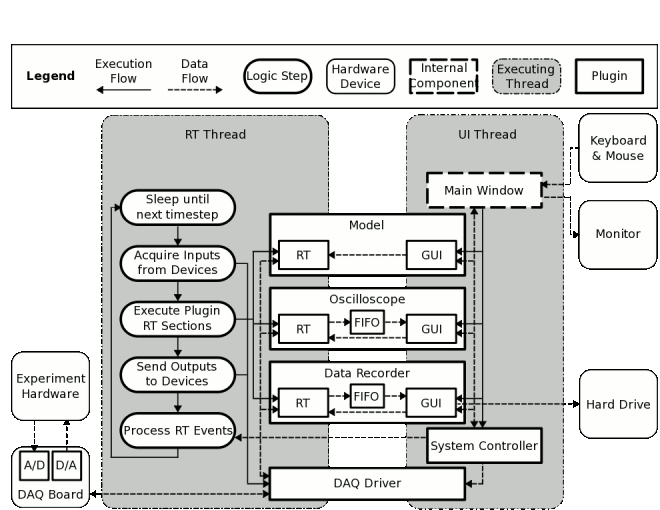
\includegraphics[width=5in]{RTXI_Block_Diagram.png} 
\caption[RTXI Architecture]{RTXI has a two-thread architecture. On every cycle, the real-time thread wakes and performs standard tasks such as sampling inputs to the DAQ card and outputting any signals. It also executes the real-time code from any loaded modules, which are dynamically linked to RTXI. The real-time thread then goes to sleep until the next cycle begins. All modules span the real-time and user interface threads.} 
\end{center}
\end{maxipage}
\end{figure}

Core system modules are not derived from the \texttt{DefaultGUIModel} class, however, and there are several different ways of implementing functionality at that level.

\begin{figure} 
\begin{maxipage}
\begin{center}
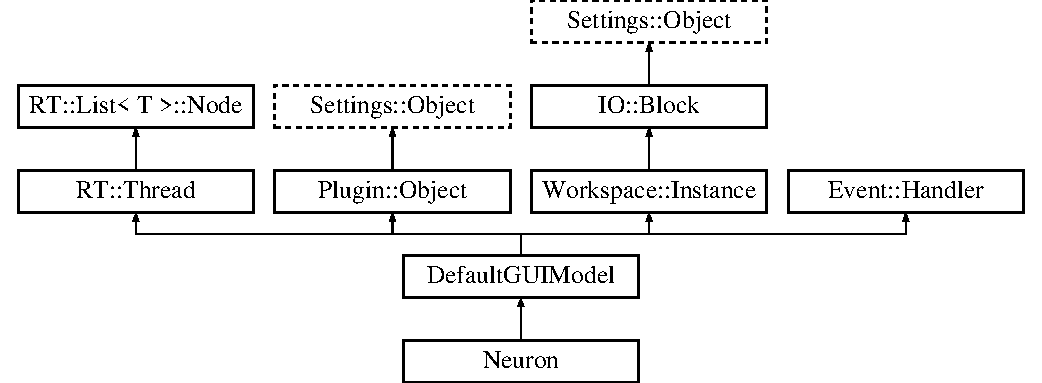
\includegraphics[width=6in]{classNeuron.pdf} 
\caption[DefaultGUIModel-derived module]{The \texttt{Neuron} module is a class derived from \texttt{DefaultGUIModel}, which inherits features such as hard real-time execution and event handling, the ability to generate and accept signals, and the ability to have metadata automatically captured by the Data Recorder to HDF5 data files.} 
\end{center}
\end{maxipage}
\end{figure}

%%%%%%%%%%%%%%%%%%%%%%%%%%%%%%%%%%%%%%%%%%%%%%%%%%%%%
\section{Software Requirements}

RTXI is a combination of several open source software initiatives:

\begin{enumerate}

\item
Linux,

\item
the Real Time Application Interface for Linux (RTAI),

\item
COMEDI,

\item
the Qt user interface framework, and

\item
HDF5.

\end{enumerate}

\marginlabel{Linux:}Linux is a generic term referring to Unix-like computer operating systems based on the Linux kernel. Their development is one of the most prominent examples of free and open source software collaboration; typically all the underlying source code can be used, freely modified, and redistributed, both commercially and non-commercially, by anyone under licenses such as the GNU General Public License. Desktop use of Linux has become increasingly user-friendly and popular in recent years. Typically, Linux is packaged into different distributions that include the Linux kernel and all of the supporting software required to run a complete system. These distributions may include modified versions of "vanilla" Linux source code and common applications, such as the vim text editor. The RTXI Live CD and manual installation notes are based on the Ubuntu desktop distribution, which is popular with new Linux users. It features a complete desktop environment with common productivity software and GUI applications for system administration.

\marginlabel{RTAI:}RTAI (http://www.rtai.org) provides real-time extensions to the official Linux kernel to make hard real-time applications possible. This is achieved by patching the kernel and introducing additional modules to handle task scheduling, capture system interrupts, etc. This requires that the kernel be recompiled and manual installation instructions are provided here. RTAI also provides several benchmark tests for evaluating your system's real-time performance.
\bigskip

\hrule
\bigskip
RTAI is not the only option for installing a real-time Linux kernel but it is the method used by the RTXI Live CD and described in the manual installation notes. RTXI also supports the Xenomai interface.
\bigskip
\hrule
\bigskip

\marginlabel{COMEDI:}\seealso{Chapter \ref{COMEDIsupport}\\COMEDI Support}The COMEDI project develops open-source drivers, tools, and libraries for data acquisition on Linux platforms. COMEDI supports a variety of common data acquisition module boards. Most RTXI users use DAQ cards by National Instruments, but any DAQ card that is supported by COMEDI should work with RTXI. RTXI can also handle multiple DAQ cards with a simple modification to the RTXI configuration file. A list of compatible DAQ cards is available in section 2.1.2.

\marginlabel{Qt:}\seealso{Chapter \ref{Qtmodules}\\Custom GUI Modules}
Qt is a cross-platform user-interface framework distributed by Nokia and used in RTXI under the LGPL license. This framework provides classes for developing sophisticated GUIs using a signals-and-slots mechanism similar to that of RTXI modules. RTXI uses Qt v3.3.8.

\marginlabel{HDF5:}\seealso{Chapter \ref{HDF5}\\Saving Data \& \\HDF5 Files}
HDF5 is a versatile data model that can represent complex data objects and a wide variety of metadata and allows you to quickly extract subsets of data. It is incorporated into RTXI through the Data Recorder module, which streams data to a HDF5 file along with the parameters of all modules connected to the Data Recorder. You can store multi-channel experimental recordings, instrument metadata, and browse images in a single file, making it possible to capture the entire collection of information about a single experiment. The format is completely portable and several tools are available for interacting with data in this format. HDFView is a free visual tool for browsing and editing HDF5 data structures and is available for Windows, Mac and Linux. MATLAB also has native functions for working with HDF5 files and we provide a tool that optimizes HDF5 files produced by RTXI for importing into MATLAB. We have developed a standardized hierarchical structure that will allow you to write MATLAB scripts that are compatible with all RTXI-generated HDF5 files.

RTXI depends on several additional Linux libraries that are typically available through the software repositories for each popular distribution of Linux:
\index{dependencies, software}
\begin{enumerate}
\item GNU Scientific Library (GSL)
\item Boost libraries
\item Qt 3.3.8
\item HDF5
\end{enumerate}